%Dies ist die Hauptseite des Dokumentes. Es werden u. a. alle Kapitel,
%Einstellung im Header eingebunden.  Veränderungen müssen in folgenden Dateien
%vorgenommen werden:
      %- Layout.tex
      %- newComments.tex
      %- Titelseite
      %- Versionsübersicht
      %- einzelne Kapitel (evtl. erweitern)


\input{einstellungen/newComments.tex}
\input{einstellungen/layout.tex}          % Diese Datei enthält alle
                                          % Layouteinstellungen

\usepackage{float}
% Dieses Befehle sortieren die Einträge in den einzelnen Listen:
%makeindex -s datei.ist -t datei.alg -o datei.acr datei.acn
%makeindex -s datei.ist -t datei.glg -o datei.gls datei.glo
%makeindex -s datei.ist -t datei.slg -o datei.syi datei.syg

% Kapitel 9
%-------------------------------------------------------------------------------

\chapter{Glossar}
Hier werden Fachbegriffe erklärt.
%% TODO: 	glossaries einpflegen.
%%		Erklährung unter: http://ewus.de/tipp-1029.html
\begin{itemize}
  \item https
  \item AFS
  \item GITZ
  \item UB
  \item sqlite
  \item \BibTeX
  \item Allegro
  \item reguläre Ausdrücke
\end{itemize}

\newcommand{\fig}[1]{
\begin{figure}[H]
    \begin{center}
        \includegraphics[width=0.8\linewidth]{bilder/#1.pdf}
        \caption{Sequenzdiagramm für allgemeine (An-)Frage-Anwort-Anweisungen}
        \label{fig:#1}
    \end{center}
\end{figure}
}

\newcommand{\zB}{\mbox{z.\,B.}\xspace}
\newcommand{\BibTeX}{\gls{glos:BibTeX}\xspace}
%------Beginn des Gesamtdokumentes----------------------------------------------
\begin{document}

%------Eingebundene Seiten, Verzeichnisse bzw. Kapitel--------------------------
% Dies ist die Titelseite des Pflichtenhefts.
% Die in "<...>" sind zu ersetzen
% Die Ausgabe darf 1 Seite nicht überschreiten, also ggf. Abstände anpassen
% Die Angabe in [...] gibt den Abstand nach der entsprechenden Zeile an.


%----Stil dieser Seite----------------------------------------------------------
\thispagestyle{plain}      % Kopfzeile bleibt leer

%----Beginn der Titelseite------------------------------------------------------
\begin{titlepage}

%----zentrierte Ausrichtung über die gesamte Seite----------------------------
\begin{center}

%----Titel des Praktikum (\praktikumTitel in newComments zu verändern)--------
{\relsize{4}{\textbf{\textsc{\praktikumTitel}}}}\\[3ex]%[5ex]

%----Titel des Teilprojektes (\projektTitel in newComments verändern)---------
{\relsize{3}{\textbf{\textsc{\projektTitel}}}}\\[3ex]%[5ex]

Software-Entwicklungspraktikum (SEP)\\
Sommersemester 2012\\[4ex]%[6ex]

{\relsize{3}\so{\textbf{Pflichtenheft}}}\\[4ex]%[5ex]

%----eingebundenes Logo der TU--------------------------------------------------
\includegraphics[scale=0.8]{bilder/carolo.jpg}\\[4ex]%[5ex]

%----Daten des Auftraggebers
Auftraggeber\\
Technische Universität Braunschweig\\
Wissenschaftliches Rechnen\\
Prof. Hermann G. Matthies\\
Hans-Sommer-Straße 65\\
D-38092 Braunschweig\\[1ex]%[2ex]
Betreuer: Elmar Zander\\[4ex]%[5ex]

% ----Tabelle der Praktikumsteilnehmer------------------------------------------
Auftragnehmer:
\begin{tabular}{l<{\hspace{20mm}} l<{\hspace{30mm}}}\\
  Name                   &   E-Mail-Adresse\\      % Zeilenüberschift
  \hline                    % Linie unterhalb der Zeilenüberschrift
  %----Nachfolgend alle Namen und E-Mail-Adressen der Teilnehmer einfügen
  Eric Anders 		& eric.anders89@web.de\\
  Johann Hong 		& johann.hong@googlemail.com\\
  Jörn Hameyer 		& j.hameyer@tu-bs.de\\
  Marco Melzer 		& marco.melzer@tu-braunschweig.de\\
  Markus Dietrich 	& markus.dietrich@tu-bs.de\\
  Philipp Offensand & PhilippOffensand@gmx.de\\
  Stephan Sobol 	& stephan.sobol@web.de\\
  Theodor van Nahl 	& t.nahl@tu-bs.de
\end{tabular}\\[1ex]%[2ex]

Braunschweig, 24.04.2012

\end{center}
\end{titlepage}
                      % Titelseite
%Diese Datei dient der Versionskontrolle. Sie ist vollständig zu bearbeiten.

%----Überschrift----------------------------------------------------------------
{\relsize{2}\textbf{Versionsübersicht}}\\[2ex]

%----Start der Tabelle----------------------------------------------------------
\begin{longtable}{|m{1.78cm}|m{1.59cm}|m{2.86cm}|m{1.9cm}|m{5.25cm}|}

  \hline                                              % Linie oberhalb

  %----Spaltenüberschriften-----------------------------------------------------
  \textbf{Version}  &    \textbf{Datum}  &    \textbf{Autor}  &
  \textbf{Status}   &    \textbf{Kommentar}       \\  %Spaltenüberschrift
  \hline                                              % Gitterlinie


  %----die nachfolgenden beiden Zeilen so oft wiederholen und die ... mit den
  %    entsprechenden Daten zu füllen wie erforderlich
  0.1    &    25.06.2012    &    Stephan Sobol,\newline Phiipp \mbox{Offensand}    &    
  in Bearbeitung    &  Kapitel 4   \\      % Eintrag in Zeile
  \hline                                                     % Gitterlinie unten
  0.2    &    25.06.2012    &    Markus Dietrich,\newline Jörn Hameyer    &    
  in Bearbeitung    &    Kapitel 3\\      % Eintrag in Zeile
  \hline                            % Gitterlinie unten
  0.3    &    25.06.2012    &    Johann Hong    &    
  in Bearbeitung    &    Kapitel 1\\      % Eintrag in Zeile
  \hline                                                     % Gitterlinie unten
  0.4    &    25.06.2012    &    Theodor \mbox{van Nahl}    &    
  in Bearbeitung    &    Kapitel 5\\      % Eintrag in Zeile
  \hline                                                     % Gitterlinie unten
  0.5    &    26.06.2012    &    Marco Melzer    &    
  in Bearbeitung    &    Kapitel 2\\      % Eintrag in Zeile
  \hline                                                     % Gitterlinie unten
  0.6    &    27.06.2012    &    Eric Anders    &    
  in Bearbeitung    &    Glossar und Rechtschreibprüfung\\      % Eintrag in Zeile
  \hline                                                     % Gitterlinie unten
  1.0    &    27.06.2012    &    sämtliche Auftragnehmer    &    
  abgenommen    &    \\      % Eintrag in Zeile
  \hline                                                     % Gitterlinie unten
  
  

%----Ende der Tabelle-----------------------------------------------------------
\end{longtable}
Status: "`in Bearbeitung"' oder "`abgenommen"'\\
Kommentar: hier eintragen, was ge\"andert bzw. erg\"anzt wurde\\

Hinweis zum Template:\\
Dieses Template enth\"alt Hinweise, die alle kursiv geschrieben sind. Alles
Kursivgeschriebene ist selbstverst\"andlich bei Abgabe zu entfernen.\\
Angaben in <...> sind mit dem entsprechendem Text zu f\"ullen.\\
\"Uberz\"ahlige Kapitel, d.h. Kapitel, die nicht bearbeitet werden m\"ussen, da
sie nicht der Aufgabenstellung entsprechen, bitte entfernen.\\

Aufgabe des Feinentwurfs:\\
Der Feinentwurf dokumentiert die klassischen Entwurfsentscheidungen wie z.B.
Verwendung bestimmter Bibliotheken oder Entwurfsmuster. Darueber hinaus
bildet der Feinentwurf die Grundlage der Implementierung, d.h. anhand
dieses Dokumentes muss jeder Softwareentwickler in der Lage sein, das Produkt
zu entwickeln. Es ist also auf Vollst\"andigkeit der Dokumentation zu
achten.
       % Versionsübersicht

\tableofcontents                          % Inhaltsverzeichnis wird automatisch
                                          % generiert
\listoffigures                            % ebenso das Abbildungsverzeichnis


%----Kapitel des Feinentwurfs, die mit Inhalt zu füllen sind--------------------
% Kapitel 1
%-------------------------------------------------------------------------------
\chapter{Einleitung}
%Hier Einleitungstext einfügen, dabei die Formatierungen selber erstellen

In diesem Feinentwurf werden die thematisierten Inhalte im Pflichtenheft und im Grobentwurf, die genaue Konstruktion eines Bibliothekmanagementsystems (WireLib), weiter konkretisiert. 
Dies erfolgt mit dem Ziel, jedem außenstehenden Softwareentwickler zu ermöglichen, die Problematik besser zu verstehen und mithilfe des Dokumentes das Projekt technisch umzusetzen.\\
Somit stehen programmspezifische Details im Vordergrund. \\
Am Anfang werden die Grundbedingungen des zu implementierenden Systems, bestehend aus den Musskriterien und den Wunschkriterien, vorgestellt.
Darauf folgt als wichtiges Element der Implementierungsentwurf: \\
Es behandelt die Dokumentation von verwendeten Klassen und Bibliotheken mit ihren entsprechenden Attributen und Methoden, unter anderem mithilfe von Klassendiagrammen sowie anderen UML Diagrammen.\\ 
Das zu verwendende Datenmodell wird im nächsten Kapitel explizit beschrieben: \\
Alle benutzten Entities und ihre Beziehungen zueinander werden näher erläutert, und sollen ein besseres Grundverständnis der Datenbank übermitteln.
Danach folgen die Betriebsanleitungen für die Serverkonfiguration.    
                % Kapitel 1
% Kapitel 2 mit den entsprechenden Unterkapiteln
% Die Unterkapitel können auch in separaten Dateien stehen,
% die dann mit dem \include-Befehl eingebunden werden.
%-------------------------------------------------------------------------------
\chapter{Analyse der Produktfunktionen}

%Dieser Abschnitt stellt die Basis für die Festlegung der Architektur dar. Die
%Festlegung einer geeigneten Architektur geschieht aufgrund der im Pflichtenheft
%analysierten Produktfunktionen und nicht-funktionalen Anforderungen, die
%realisiert werden müssen. Jede betrachtete Funktion wird in einem eigenen
%Unterkapitel dokumentiert.  Fügen Sie bitte so viele Unterkapitel ein, wie
%Produktfunktionen im Pflichtenheft vorhanden sind. Auch die nicht-funktionalen
%Anforderungen sind so weit möglich entsprechend darzustellen.
%
%
%\section{Analyse von Funktionalität <ID aus Pflichtenheft>: <Funktionsname>}
%z.B.: Analyse von Funktionalität /F10/: Automatisches Einlagern
%In diesem Abschnitt wird die im Titel angegebene Produktfunktion sowohl im
%Hinblick auf ihre Verteilung auf die Architektur als auch im Hinblick auf die
%zu ihrer Realisierung nötigen Datenstruktur untersucht.  Zu Beginn die
%Funktionalität kurz beschreiben.  Anschließend erfolgt die Darstellung der
%Realisierung der Funktion als Interaktion von Komponenten des zu entwickelnden
%Systems in einem Sequenzdiagramm. Das Diagramm bitte ebenfalls kurz
%beschreiben.
Im folgenden werden die Funktionen und Qualitätsmerkmale des System auf ihre
Modulzugehörigkeit hin geprüft und eingeordnet. Dabei wird auf das
Basis-Konstrukt von Django aufgebaut und die Funktionen bzw. Qualitätsmerkmale
werden in unterschiedliche Kategorien eingeteil.

Hier zuerst die Kategorienen in die, Die einzelnen Funktionen und
Qualitätsmerkmale eingeordnet werden.
\begin{itemize}
	\item Build in Django
	\item Model einer Django-App
	\item Klassen bzw. Objectmethode
	\item Template
	\item View im Backend
	\item View im Frontend
\end{itemize}

%% Aufgaben: 
% Kapitel 1 bearbeiten
\section{Analyse von Funktion F100: Anmeldung}
Der Benutzer meldet sich auf dem System unter seinem Benutzernamen an.

Diese Funktion, die lediglich in der Komponente \textbf{View} vorkommt, ist
eine Built-in-Funktion von \gls{glos:django}. Innerhalb von Django werden die Benutzer
in einer eigenen Datenstruktur  dargestellt. Diese Klasse muss erweitert werden,
um die zusätzlichen Daten der Benutzer zu speichern. Da \gls{glos:django} eine Datenbank
zugrunde liegt, müssen diese weiteren Daten in einer extra Klasse mit Referenz
auf die Benutzer gesetzt werden.

\section{Analyse von Funktion F101: Anmeldung über LDAP}
Der Benutzer meldet sich auf dem System über seinen \Gls{GITZ}-Benutzer (\zB
y-Nummer) an und hat seinem internen Status folgend entsprechende Rechte auf dem
System.

Diese Funktion wird in einer extra App dargestellt. Die \gls{LDAP}-Anmeldung muss
dabei die normale Anmeldung erweitern und im View evtl. durch eine Checkbox zur
Verfügung gestellt werden. Die zugrundeliegende Datenstruktur wird von \gls{LDAP}
bereit gestellt.

\section{Analyse von Funktion F102: Anbindung an die Universitätsbibliothek}
Ein Benutzer mit hinreichenden Rechten erzeugt über das Frontend des Produktes
eine Datei mit den aktuell zu exportierenden Daten. Nach der Generierung steht
dem Benutzer eine Datei im \gls{glos:allegro}-Format zur Verfügung, die er
manuell an die \gls{UB} weiterleiten kann.

Der zugrunde liegende Datensatz der Dokumente wird von einem, in den
\textbf{Models} gelegenen Befehlssatz in ein Datenformat übersetzt, welches von
der TU Braunschweig Universitätsbibliothek gelesen werden kann. 

\section{Analyse von Funktion F103: Mailtexte ändern}
Die Standard-Mails, die vom System an Benutzer verschickt werden, sollen geändert
werden.

Die Mailtexte sind Bestandteil einer veränderbaren, aber nicht großen Tabelle an
Basisinformationen, wie auch andere Einstellungen für die Software. Um die
Informationen bereit zu stellen, muss eine neue Klasse in den \textbf{Models}
erzeugt werden, die alle Informationen für die App bereit stellt.

\section{Analyse von Funktion F200: Bib\TeX\ Import}
Ein oder mehrere Dokumente werden zum System hinzugefügt. Dafür wählt der
Benutzer den entsprechenden View aus und lädt über einen Upload-Dialog eine
\BibTeX -Datei hoch. Das System analysiert die Datei auf Validität, erzeugt
Objekte aus den Daten, die in eine Datenbank gespeichert werden.

Für die Funktion wird also ein \textbf{View} benötigt, der den Upload bereit
stellt.  Als Basis werden die Dokument-Objekte aus den \textbf{Models} benötigt,
die auch von vielen weiteren Funktionen verwendet werden und die auch über
\gls{glos:django} die Datenbankeinträge verwalten.
 % Q10 zusätzlich! %% Theo
\section{Analyse von Funktion F201: Webinterface-Import}
\label{f:201}
Der Benutzer, der entsprechende Rechte hat, wählt einen View, der ein Interface
bietet, um die Daten für einzelne Dokumente in das System einzupflegen. Dafür
wird ihm vom System ein Formular auf dem View angeboten, in dem er alle
Informationen zu einem Buch eintragen kann.

Als Teil der Komponente \textbf{View} stellt diese Funktion für den
Benutzer eine weitere Schnittstelle zur internen \BibTeX -Verwaltung zur Verfügung. Es wird
daher ein Zugriff auf die Komponente der \textbf{Models} benötigt.

\smallfig[Webinterface-Import]{f201}
Wie in der Grafik \ref{fig:f201}\ zu erkennen, wird von dem Benutzer durch das
Absenden seines Formulars der Import in die Datenbank eingeleitet. Nach
Abschluss dieses Vorganges wird dem Benutzer ein entsprechender Status zurück
geliefert.

\section{Analyse von Funktion F202: Editieren von Dokumenten}
Der Benutzer, der entsprechende Rechte hat, nimmt auf der Detailansicht eines
Dokumentes die Möglichkeit wahr, die Daten dieses Dokumentes nachträglich zu
ändern. Dafür wählt er die entsprechende Option und wird vom System auf eine
Seite ähnlich der aus \ref{f:201} \nameref{f:201} mit einer ausgefüllten Maske
geleitet.

\fig[Editieren von Dokumenten]{f202}
Diese Funktion muss zu erst das Dokument auslesen, um den View zu erzeugen und
dann die Einträge des Dokumentes entsprechend zu ändern. Eine solche Veränderung
von den Objekten benötigt lediglich entsprechende set- und get-Methoden für die
Dokumente und einen entsprechenden View für \gls{glos:django}. Der in der
\textbf{DB} zugrundeliegende Datensatz wird also über \textbf{View} mit
den \textbf{Models} manipuliert. Der Verlauf dieser Funktion wird in der Grafik
\ref{fig:f202}\ dargestellt.


\section{Analyse von Funktion F203: Löschen von Dokumenten}
Der Administrator, als einziger Benutzer mit den entsprechenden Privilegien,
löscht ein Dokument vollständig aus der Datenbank inkl. der Ausleihhistory.
Diese Aktion wird über einen View im Backend erledigt, der dort bereit steht.

\smallfig[Löschen von Dokumenten]{f203}

Benötigt wird für \gls{glos:django} ein entsprechender \textbf{View} im Backend, der die
Möglichkeit bietet, die eingetragenen Dokumente im Backend einzusehen. Weiter
wird die zugrundeliegende Funktion der Löschung von Objekten aus der Datenbank
in den \textbf{Models} benötigt, die zur Basis in \gls{glos:django} bereits Built-In ist,
jedoch evtl. erweitert werden muss.

\section{Analyse von Funktion F210: Generelle Suche}
Der Benutzer gibt in eine Suchmaske einen oder mehrere Begriffe ein, um seine
Suche zu spezifizieren. Nach der Bestätigung der Eingabe gibt das System
entsprechende Treffer dem Benutzer in einer Liste zurück.

\smallfig[Generelle Suche]{f210}

Die zugrundeliegenden Funktionen der Objekt-Suche nach bestimmten Parametern
wird bereits durch \gls{glos:django} bereit gestellt. Der Such-View arbeitet dabei auf
einer Funktion, die für die Dokumentfunktionen arbeitet.
 %% Theo
\section{Analyse von Funktion F210 (Generelle Suche)}
Diese Funktion ist eine Build-In Funktion von Django. Das gesuchte Wort wird einfach mithilfe einer Search-Query innerhalb der Datenbank gesucht und ausgegeben. 

\section{Analyse von Funktion F211 (Suche mit erweiterten Ausdrücken)}
Auch diese Suche wird von Django mithilfe von mehreren Querysets bereitgestellt und ist daher bereits eine Built-In Funktion.

\section{Analyse von Funktion 212 (erweiterte Suche)
Im FrontEnd werden die bestätigten Parameter (aus der Maske für die erweiterte Suche) den dazu passenden Built-In Querysets im System übergeben. 

\section{Analyse von Funktion 213 (Suche mit regulären Ausdrücken)
Diese Funktion muss in einer extra App dargestellt werden, wo genau bestimmt wird, welche aus der FrontEnd ermittelten Zeichenfolgen in der Suchanfrage bestimmte Querysets auslösen.

\section{Analyse von Funktion 214 (Sortierung der Suche)
Auch diese Funktion muss in einer extra App dargestellt werden. Das vorläufige Ergebnis aus einer Suchanfrage wird tabellarisch angezeigt, dessen Spalten aber interaktiv sind: Die Spaltennamen lösen system-intern Funktionen aus, die aus Build-In Querysets bestehen, die genau bestimmen, wie die Ergebnisse dargestellt werden sollen (in diesem Fall alphabetisch aufwärts/abwärts). 



 
\section{Analyse von Funktion F220: Ausleihe}
\label{f:220}
Ein oder mehrere Dokumente werden von einem Benutzer ausgeliehen. Dabei wählt der Benutzer die gewünschten Dokumente aus und das System muss in der Datenbank nachprüfen, ob diese derzeit ausleihbar sind. Der Status des Dokumentes müsste also \"0\" sein. Wenn dies der Fall sein sollte, werden dem Benutzer diese Bücher zugewiesen. Dies erfolgt durch zwei Built-In-Funktion von Django mit dessen Hilfe die Datenbank erweitert bzw.\ ein Datensatz geupdatet werden kann.

\section{Analyse von Funktion F221: Ausleihe an Externe}
Die Ausleihe an Externe ist ähnlich gestaltet wie in \ref{f:220}\nameref{f:220}. Es existiert lediglich der Zusatz, dass der Benutzer einen Externen als eigentlichen Ausleiher angibt. Dafür wird beim Entleihen die Möglichkeit gegeben Daten über den Externen anzugeben, dessen Daten dann gespeichert und beim Entleihen vermerkt werden. Auch hierbei wird eine Built-In-Funktion zum erweitern der Datenbank genutzt.

\section{Analyse von Funktion F222: Ausleihe übertragen}
Ein Dokument wechselt den Ausleihenden. Dabei muss ein Benutzer $A$ ein von ihm ausgeliehenes Dokument auswählen und einem anderen Benutzer $B$ übertragen. Alternative kann Benutzer $B$ auch eintragen, dass er sich ein Dokument von Benutzer $A$ geholt hat, das Dokument also jetzt bei ihm zu finden ist. Das System vermerkt dieses Austausch dann in der Datenbank mittels einer Built-In-Funktion von Django. 

\section{Analyse von Funktion F223: Ausleihe zurückgeben}
Ein Benutzer braucht ein Dokument nicht mehr und gibt es in den Bestand der Bibliothek zurück. Auch hierfür muss der Benutzer als Entleiher des Dokumentes eingetragen sein. Wenn dies der Fall sein sollte, kann er \emph{zurückgeben} wählen und das Dokument wird auch im Datensatz mittels Built-In-Funktionen von Django mit dem Status \"0\" versehen.

\section{Analyse von Funktion F224: (Optional) Ausleihe vermisst melden}
Das Dokument befindet sich nicht mehr an dem laut Datenbank befindlichen Ort. Dann kann ein Benutzer ein Dokument auf der Dokumentenansicht als \emph{vermisst} melden und dieses wird in der Datenbank mittels Statusänderung vermerkt. Dazu wird eine E-Mail an alle Benutzer verschickt oder alternativ eine Meldung auf der Homepage angezeigt. Hierfür muss eine neue App erstellt werden, die den Status ändert, die E-Mail-Adressen, den -Text und die Dokumentinformationen aufruft, verarbeitet und an alle verschickt oder alternativ einen entsprechenden Beitrag auf der Homepage erstellt.

\section{Analyse von Funktion F225: Ausleihe verloren melden}
Das Dokument ist auch nach einer Vermisstenmeldung nicht wieder aufgetaucht. Dann ist ein Bibliothekar berechtigt, es als \emph{verloren gegangen} einzustufen. Das Dokument bekommt den entsprechenden Status und wird demnächst bei weiteren Suchanfragen ausgeschlossen. Dies erfolgt wieder durch eine Built-In-Funktion von Django.
\section{Analyse von Funktion F226: Ausleihfrist abgelaufen}
Falls die Leihdauer eines Dokumentes abgelaufen ist, wird der Mailtext aus der 
Datenbank abgerufen und an die E-Mail Adressen der beiden Entleiher(Bürge/Entleiher) gesendet.

Hierfür muss eine neue App erstellt werden, welche alle benötigten Informationen enthält bzw. sich aus der Datenbank holt, um diese Funktion zu bewerkstelligen.
Diese Funktion gehört zur Komponente \textbf{Models}, natürlich in Interaktion mit \textbf{DB}.


\section{Analyse von Funktion F227: Ausleihhistory}
Die Ausleihhistory ist eine Liste von Personen, welche bereits ein bestimmes Buch ausgeliehen hatten bzw. immer noch haben.
Es wird ein Filter über die Dokument-Objekte gelegt, damit nur bestimmte bzw. die gewünschten Dokumente und deren bisherige Ausleiher ausgegeben werden. Diese so erhaltenen Daten müssen nun noch durch ein Frontend-View an geigneter Stelle der Web-Seite angezeigt werden.
Diese Funktion ist eine Built-In-Funktion von Django und wird über \textbf{View} benutzt. Da die Informationen wiederrum nur in der Datenbank liegen, muss diese Komponente bei jeder Anfrage auf \textbf{DB} zugreifen.
Das Sequenz-Diagramm wird hier nicht dargestellt, da es eine einfache Suchanfrage an die DB mit anschließendem, gefilterten Ergebnis ist, siehe auch 

\section{Analyse von Funktion F228: Derzeitiger Leihender}
Die Funktion Derzeitiger Leihender gibt die Person aus, welche grad ein bestimmes Buch ausgeliehen hat.
Da in Django die User durch eine eigene Klasse dargestellt werden, muss diese Klasse auf die Rechte des momentan angemeldeten Benutzers überprüft werden. Falls diese Rechte ausreichend sind, wird wiederum durch ein Queryset+Filter die jeweiligen Dokumente und der dazugehörige Leihende durch einen View ausgegeben.
Auch diese Funktion benutzt die Komponente \textbf{View} in Zusammenhang mit \textbf{DB} (siehe auch \ref{f:227} \nameref{f:227}).
Auch hier wird auf eine Angabe des Sequenzdiagrammes verzichtet, da es wie auch in \ref{f:227} \nameref{f:227} eine einfache gefilterte Suchanfrage ist.



\section{Analyse von Funktion F229: Entleihliste}
Wenn der Benutzer angemeldet ist, ist er im Stande, sich alle seine momentan entliehene Dokumente als Liste anzeigen zu lassen.

Diese Funktion greift auf die Komponente \textbf{View} zu, um die Informationen dafür zu erhalten, muss vorher jedoch auf die \textbf{DB} zugegriffen werden.
Das Sequenzdiagramm für diese Funkton wird hier nicht angegeben, siehe \ref{f:227} \nameref{f:227} oder \ref{f:228} \nameref{f:228}.

\section{Analyse von Funktion F230: Bib\TeX -Export}
Diese Funktion gehört zur Komponente \textbf{View:Export}. Die für diesen Export nötigen Informationen sind vollständig in der Datenbank enthalten und müssen mit \gls{glos:django} ermittelt werden. Die so erhaltenen Daten werden dem Benutzer in einer View im \BibTeX -Format zum Kopieren angezeigt. Verdeutlicht wird dies in dem Sequenzdiagramm \ref{fig:BibTeX-Export}.

\begin{figure}[H]
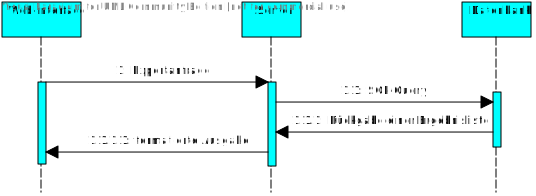
\includegraphics[width=0.8\linewidth]{bilder/Seq-BibTex.pdf}
\caption[BibTeX-Export]{BibTeX-Export}
\label{fig:BibTeX-Export}
\end{figure}

\section{Analyse von Funktion F231: Universitätsbibliothek-Export}

Diese Funktion muss in einer extra Klasse dargestellt werden. Die für diesen
Export nötigen Informationen sind vollständig in der Datenbank enthalten und
müssen mittels \gls{glos:django} ermittelt werden. Diese Daten
werden durch eine Funktion in das richtige Format gebracht und in einem vom
Benutzer vorher gewählten Dateipfad in einem Allegro kompatiblen Format
gespeichert. Diese Komponente gehört ebenfalls zur Komponente
\textbf{View:Export}. Veranschaulicht wird der Vorgang in dem Sequenzdiagramm
\ref{fig:Allegro-Export}.

\begin{figure}[H]
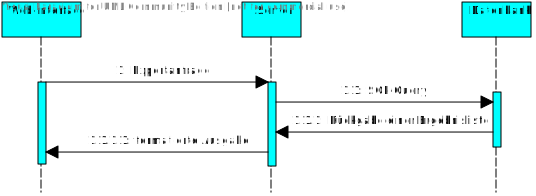
\includegraphics[width=0.8\linewidth]{bilder/Seq-BibTex.pdf}
\caption[Allegro-Export]{Allegro-Export}
\label{fig:Allegro-Export}
\end{figure}

\section{Analyse von Funktion F300: Benutzerverwaltung}
Alle Informationen zu den Benutzern werden in einer Datenbank gespeichert. Änderungen an bestehenden Benutzern und das Hinzufügen neuer Benutzer wird durch ein Webformular von einem Benutzer mit ausreichenden Rechte eingeleitet. Mithilfe von \gls{glos:django} werden die Informationen aus dem Formular gelesen und alle Änderungen in der Datenbank eingetragen. Das Sequenzdiagramm ist trivial, da nur einfach Frage/Antwort-Vorgänge zwischen Server und Datenbank stattfinden. Diese Komponente gehört zur Komponente \textbf{Admin}.

\begin{figure}[H]
  \begin{center}
	\includegraphics[width=0.6\linewidth]{bilder/f300.pdf}
	\caption[Benutzerverwaltung]{Benutzerverwaltung}
	\label{fig:300}
  \end{center}
\end{figure}

In dem Diagramm sieht man, dass zuerst die Rechte als Dateneingabe in das
System gegeben werden, diese dann an den Server weitergegeben werden. Der
Server richtet dann die Änderungsanfrage an die Datenbank und bekommt entweder
eine Bestätigung oder eine entsprechende Fehlermeldung, die er an das
Web-Interface zurückgibt.

\section{Analyse von Funktion F301: Rechtezuweisung für Rollen}
Die Rechte einer Rolle werden in einer eigenen Tabelle der Datenbank gespeichert. Ein Benutzer mit ausreichenden Rechten kann über ein Webformular Änderungen eingeben. Diese Änderungen werden mithilfe von \gls{glos:django} aus dem Webformular ausgelesen und in der Tabelle der Datenbank gespeichert. Das Sequenzdiagramm ist trivial, da nur einfach Frage/Antwort-Vorgänge zwischen Server und Datenbank stattfinden. Diese Funktion gehört zur Komponente \textbf{Admin}.


\begin{figure}[H]
  \begin{center}
	\includegraphics[width=0.6\linewidth]{bilder/f300.pdf}
	\caption[Rechtezuweisung für Rollen]{Rechtezuweisung für Rollen}
	\label{fig:301}
  \end{center}
\end{figure}

In dem Diagramm sieht man, dass die Änderungen der Rollenrechte zuerst im
Web-Interface eingegeben werden und diese als Datenpaket an den Server
übermittelt. Dieser wertet die Daten aus und stellt eine entsprechende
Änderungsanfrage an die Datenbank. Er verarbeitet die aus einer Fehlermeldung
oder einer Bestätigung bestehende Antwort und gibt eine entsprechende
Ausgabemeldung an das Web-Interface zurück.

\section{Analyse von Funktion F302: Benutzer Rolle(n) zuweisen}
Die Rollen eines Benutzer werden in einer speziellen Tabelle in der Datenbank gespeichert. Ein Benutzer mit ausreichenden Rechten kann über ein Webformular Änderungen eingeben. Diese Änderungen werden mithilfe von \gls{glos:django} aus dem Formular ausgelesen und in der entsprechenden Datenbank gespeichert. Das Sequenzdiagramm ist trivial, da nur einfach Frage/Antwort-Vorgänge zwischen Server und Datenbank stattfinden. Diese Funktion gehört zur Komponente \textbf{Admin}.

\begin{figure}[H]
  \begin{center}
	\includegraphics[width=0.6\linewidth]{bilder/f302.pdf}
	\caption[Benutzer Rolle(n) zuweisen]{Benutzer Rolle(n) zuweisen}
	\label{fig:302}
  \end{center}
\end{figure}

In dem Sequenzdiagram sieht man, dass die Änderungen an der Relation zuerst im
Web-Interface eingegeben und dann an den Server übermittelt werden. Dieser
überprüft sie und schickt eine passende Änderungsanfrage an die Datenbank.
Diese verarbeitet die Anfrage und gibt dem Server entweder eine Bestätigung
oder eine Fehlermeldung zurück, die dieser in eine Ausgabe umwandelt und an das
Web-Interface weiterreicht.


\section{Analyse von Qualitätsmerkmal /Q10/ (Sicherheit der Anmeldung)}
Die Verschlüsselung der Anmeldung wird von Django bereit gestellt und ist daher
bereits eine Build-In-Funktion. 
\section{Analyse von Qualitätsmerkmal /Q11/ (SQL-Injections vermeiden)}

%% TODO
SQL-Statements werden ausschließlich durch Übergabe von Parametern an 
Funktionen von Django ausgeführt. SQL-Injections sind in Django durch 
integriertes Escaping von SQL-Syntax nicht möglich. Nur wenn RAW-SQL 
ausgeführt werden soll, oder aber an die Funktion .extra von Django 
übergeben werden soll, ist eigenes Escaping notwendig.

\section{Analyse von Qualitätsmerkmal /Q20/ (Layoutstruktur)}

%% TODO
% Glossareintrag hinzufügen.
Die Templates für Django müssen so angepasst werden, dass sie dem Corporate
Design der TU Braunschweig entsprechen. Dies wird durch Verwendung ensprechender
Grafiken, Cascading-Stylesheets, Webseitenstruktur und weiteren Mitteln erreicht.


\section{Analyse von Qualitätsmerkmal /Q21/ (Klare Struktur)}

%% TODO
Die Stylesheets für die Templates von Django sowie die Templates selber
müssen so konstruiert werden, dass der auf der Webseite dargestellte 
Inhalt übersichtlich ist. Menüführung soll ebenfalls ohne Verschachtelung
möglich sein. Ein entsprechendes Design muss vorher entworfen werden.


\section{Analyse von Qualitätsmerkmal /Q22/ (Suche)}

%% TODO
% Beschreibung hinzufügen

Verwendet wird die in Django bereits implementierte Suche. Diese Suche ist ohne
große Anpassungen bereits intuitiv und einfach nutzbar.


\section{Analyse von Qualitätsmerkmal /Q30/ (Zeichenketten)} 

%% TODO
Die Bearbeitung von Zeichenketten als Unicode wird bereits von der benutzten
Datenbank SQLite erfordert, welche nur Unicode-codierte Zeichenketten benutzt.


\section{Analyse von Qualitätsmerkmal /Q31/ (Löschen von Dokumenten)} 

Löschen von Dokumenten ist mit Django möglich. Intern muss verhindert werden,
dass andere Nutzer als Administratoren löschen dürfen.

  % Kapitel 2
% Kapitel 3 mit den entsprechenden Unterkapiteln
% Die Unterkapitel können auch in separaten Dateien stehen,
% die dann mit dem \include-Befehl eingebunden werden.
%------------------------------------------------------------------------------------
\chapter{Resultierende Softwarearchitektur}

%Dieser Abschnitt hat die Aufgabe, einen Überblick über die zu entwickelnden
%Komponenten und Subsysteme zu liefern.
\section{Komponentenspezifikation}

%In diesem Abschnitt wird die aus der Analyse der Produktfunktionen (Kapitel 2)
%resultierende Komponentenstruktur zunächst überblickartig durch ein
%Komponentendiagramm beschrieben. Die Bezeichnungen und Anzahl der Komponenten
%muss natürlich konsistent sein mit der in Kapitel 2!
Bei der Analyse der notwendigen Komponenten fallen drei Komponentenbereiche auf.
Zum einen muss der Client beachtet werden, zum anderen gibt es den Server. Der
Server besteht aus der \gls{glos:django}-App, den Templates und der Datenbank. Die App
benötigt noch die Views und den Adminbereich zur Kommunikation mit dem Client
und die Models für den Zugriff auf die Datenbank.

\begin{figure}[h]
    \begin{center}
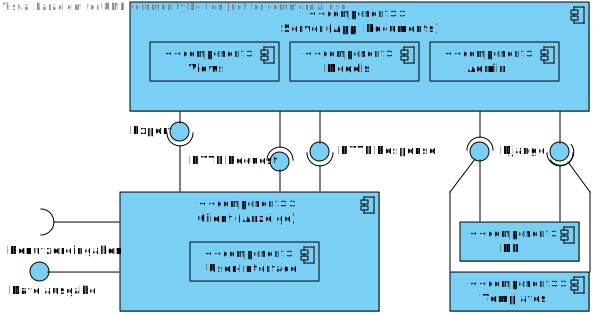
\includegraphics[width=0.8\linewidth]{bilder/Komponentendiagramm.pdf}
\caption[Komponentendiagramm]{Komponentendiagramm}
\label{Komponentendiagramm}
    \end{center}
\end{figure}

\section{Schnittstellenspezifikation}

\begin{tabular}[ht]{|l|p{0.35\linewidth}|p{0.35\linewidth}|}
\hline
Schnittstelle & \multicolumn{2}{|c|}{Aufgabenbeschreibung}\\
\hline
\hline
/S10/ HTTP Request & \multicolumn{2}{|c|}{}\\
\hline
& search(String) : List & Die Suche liefert eine Liste mit den Ergebnissen\\
& signIn(String) : boolean & Anmelden des Benutzers\\
& signOut() : boolean & Abmelden des Benutzers\\
& import(data) : boolean & Import \\
& getHistory(String) : List & liefert eine Liste der Ausgeliehen Dokumente\\
& getDoc(String) : List & liefert die Dokumentinformationen in einer Liste\\
& getView(String) : View & liefert die View, die die Aufgabenstellung erfüllt\\
\hline
/S20/Export & \multicolumn{2}{|c|}{Exportieren von Informationen}\\
\hline
& exportBibTeX() : String & Liefert einen String welcher die
Dokumentinformationen im \BibTeX -Format enthält\\
& exportAllegro() : \Gls{glos:Allegro} -kompatible Datei & Liefert eine Datei für die
\Gls{UB}\\
\hline
/S30/\gls{glos:django} & \multicolumn{2}{|c|}{Verbindung mit Datenbank}\\
\hline
& connect(String) : boolean & Verbindung zur Datenbank\\
& disconnect() : boolean & Verbindung wird beendet\\
& sendQuery(String) : List & liefert eine Liste des Ergebnisses\\
\hline
\end{tabular}





\section{Protokolle für die Benutzung der Komponenten}

In diesem Unterkapitel werden nun die Protokoll-Statecharts für alle 
Komponenten, welche in dem Komponentendiagramm \ref{Komponentendiagramm} 
vorhanden sind, dargestellt.

Für jede dieser Komponenten ist eine Wiederverwendung begrenzt sinnvoll, da alle
 diese Komponenten sehr projektspezifisch gehalten werden müssen. Sie können 
 unter Umständen in anderen Projekten eingesetzt werden, aber dann nur unter 
 größtem Anpassungsbedarf.

\subsection{Client}
\begin{figure}
\includegraphics[width=0.8\linewidth]{bilder/KompClient.pdf}
\caption{Statechart für die Komponente Client}
\label{StClient}
\end{figure}

Vom Startzustand des Statecharts Abb.\ \ref{StClient} aus gibt es entweder die 
Möglichkeit, dass der Client eine Djangoview oder die Adminansicht aufruft. Wird 
die Adminkomponente aufgerufen, erwartet der Client zuerst eine 
Authentifizierung. Schlägt diese fehl, wird der Zugriff verweigert. Wenn sie 
aber erfolgreich ist, erwartet der Client als nächstes ein oder mehrere 
Adminaktionen oder das Beenden der Adminansicht. Ruft der Client eine Djangoview 
auf, lädt er zuerst die entsprechende View und stellt dann einen HTTP-Request. 
Sobald er das entsprechende Ergebnis erhält, gibt er es aus und lädt benötigte 
Javascripte. Damit ist die Seite komplett geladen und der Client in seinem 
Endzustand.

\subsection{View}
\begin{figure}
\includegraphics[width=0.8\linewidth]{bilder/KompView.pdf}
\caption{Statechart für die Komponente View}
\label{StView}
\end{figure}

Eine View (Statechart Abb.\ \ref{StView}) erhält immer zuerst einen HTTP 
Request, den sie lädt und dann verarbeitet. Ist dies geschehen, wird über das 
Djangotemplatesystem eine entsprechende fertige Webseite erzeugt und per HTTP 
Response zurückgegeben. Alternativ kann die Rückgabe auch aus einem Fehler 500 
bestehen.

\subsection{Model}
\begin{figure}
\includegraphics[width=0.8\linewidth]{bilder/KompModel.pdf}
\caption{Statechart für die Komponente Model}
\label{StModel}
\end{figure}

Nachdem das Objekt initialisiert ist, kann entweder eine Anfrage oder eine
Bearbeitung ausgeführt werden (siehe Statechart Abb.\ ref{StModel}). Wird etwas 
bearbeitet, werden die Daten zuerst in ein DB-kompatibles Format geändert. 
Nachdem DB-Insert werden die Daten noch im Arbeitsspeicher gehalten, bis der 
Commit abgeschlossen ist und die Daten konsistent gemacht wurden. Dann löscht 
der Garbage Collector das Objekt und versetzt es damit in seinen Endzustand. 
Wurde eine Anfrage gestellt, werden die Daten entsprechend der Query geladen. 
Nach der Verarbeitung der Daten und der Erstellung des Ergebnisses der Query 
wird dieses in einer Ausgabe dargestellt. Nachdem die Ausgabe beendet wurde, 
wird das Objekt vom Garbage Collector gelöscht und damit in seinen Endzustand 
versetzt.

\subsection{Admin}
\begin{figure}
\includegraphics[width=0.8\linewidth]{bilder/KompAdmin.pdf}
\caption{Statechart für die Komponente Admin}
\label{StAdmin}
\end{figure}

Die Komponente Admin (Abb.\ \ref{StAdmin}) erstellt zuerst eine Webseite, dann 
initialisiert sie entprechende Objekte und registriert sie. Damit ist die 
Adminseite vollständig geladen. Die restliche Funktionsweise wurde bereits in 
Abb.\ \ref{StClient} beschrieben, da diese ineinander greifen.


\subsection{DB und Template}
Die Komponente \textbf{DB} wird hier nicht modelliert, da diese zunächst trivial
 ist(Anfrage an DB -> DB liefert Ergebnis) und die \textbf{DB} vollkommen durch 
 \gls{glos:django} auf die Komponente \textbf{Models} gemappt wird.

Auch auf eine Darstellung der Komponente \textbf{Template} wird verzichtet, da 
ein Template nur einen wirklichen Zustand hat, und dies ist der des Existierens. 




%In diesem Abschnitt wird mit Hilfe von Protokoll-Statecharts die korrekte
%Verwendung der zu entwickelnden Komponenten dokumentiert. Dies ist insbesondere
%für diejenigen Komponenten notwendig, für die eine Wiederverwendung möglich
%erscheint oder sogar bereits geplant ist.

%Begründen Sie für welche Komponenten eine Wiederverwendung sinnvoll erscheint
%und für welche nicht!

%Fügen Sie so viele Statechartdiagramme ein, wie sie Komponenten gefunden haben.
      % Kapitel 3
% Kapitel 4
%-------------------------------------------------------------------------------
\chapter{Verteilungsentwurf}
Da es sich bei dem Produkt um eine Datenbank-basierte Webanwendung handelt, liegt hier ein verteiltes System in Form eines Client-Server-Modells vor:

\begin{figure}[h]
\includegraphics[width=0.8\linewidth]{bilder/Webanwendung2.png}
\caption{Client-Server-Modell}
\label{Client-Server-Modell}
\end{figure}

Durch eine Ressource-Anforderung (request) mithilfe eines Webbrowsers benutzt der Client über eine IP (oder einem Servernamen) die Adresse des Servers. Dieser gibt den Request an den Webserver weiter.
Mithilfe des Servers beanwortet der Webserver schließlich den Request und schickt das Ergebnis (response) an den Client zurück.   

        % Kapitel 4

%---Hier werden das Glossar und das Abkürzungsverzeichnis gedruckt--------------
\providetranslation{Glossary}{Glossar}
\printglossary[style=altlist,title=Glossar]

\providetranslation{Acronyms}{Akronyme}
\printglossary[type=\acronymtype,style=long]


%------Ende des Dokumentes------------------------------------------------------
\end{document}

